%\title{Исследование производственных систем с маршрутизацией, зависящей от состояния}
%\author{Салин Роман Владимирович}
%\institute{САРАТОВСКИЙ ГОСУДАРСТВЕННЫЙ УНИВЕРСИТЕТ ИМЕНИ Н.Г. ЧЕРНЫШЕВСКОГО}
%\date{Саратов, 2014}

\begin{frame}[plain]
\begin{center}
Министерство образования и науки Российской Федерации\\
САРАТОВСКИЙ ГОСУДАРСТВЕННЫЙ УНИВЕРСИТЕТ\\
ИМЕНИ Н.Г. ЧЕРНЫШЕВСКОГО
\end{center}

%\vspace{0.5cm}
%\begin{flushright}
%\parbox{6.8cm}{
%\raggedright
%  Кафедра системного анализа \\ и автоматического управления
%}
%\end{flushright}

\vfill

\begin{center}
\textbf{Исследование производственных систем с маршрутизацией,\\зависящей от состояния}\\
\medskip
ВЫПУСКНАЯ КВАЛИФИКАЦИОННАЯ РАБОТА СПЕЦИАЛИСТА
\end{center}
\begin{flushleft}
студента 5 курса 511 группы\\
специальности 010501 --- прикладная математика и информатика\\
факультета компьютерных наук и информационных технологий\\
Салина Романа Владимировича
\end{flushleft}

\vfill

\noindent
\begin{flushleft}
Научный руководитель\\
доцент, к.ф.-м.н. \hfill В. И. Долгов\\
\end{flushleft}

\vfill

\begin{center}
Саратов 2014
\end{center}
\end{frame}

% ------------------------------------------------------------------- %

\begin{frame} \frametitle{Цели и задачи дипломной работы}
\begin{itemize}
\item исследование производственных систем с маршрутизацией, зависящей от состояния;
\item разработка алгоритма метода анализа производственных систем с маршрутизацией, зависящей от состояния;
\item программная реализация алгоритма;
\item проведение численных экспериментов с разработанной программой
\end{itemize}
\end{frame}

% ------------------------------------------------------------------- %

\begin{frame} \frametitle{Гибкие производственные системы}
$C_i$ --- множество рабочих станций (систем), $i \in I \equiv \{ i ~|~ i=1,...,L \}$;

$t$ --- множество типов производственных операций, $t \in T$;

$\kappa_i$ --- параллельно работающие машины (приборы) на станции $C_i$;

$s_i$ --- емкость рабочей станции, $s_i \geqslant \kappa_i, ~ i=1,...,L$;

$\kappa = (\kappa_i)$ --- вектор числа приборов на рабочих станциях, $i=1,...,L$;

$s = (s_i)$ --- вектор емкостей рабочих станций, $i=1,...,L$.

$C_0$ --- система транспортировки материалов (MHS);

$\kappa_0$ --- транспортеры в $C_0$;

$N$ --- общее число деталей, $N \leqslant \sum\limits_{i=1}^L s_i$.
\end{frame}

% ------------------------------------------------------------------- %

\begin{frame} \frametitle{Гибкие производственные системы}
\begin{figure}[H]
  \centering
  \includegraphics[width=0.9\textwidth]{fms}
  \label{fig:main}
\end{figure}
\end{frame}

% ------------------------------------------------------------------- %

\begin{frame} \frametitle{Гибкие производственные системы}
$N_t$ --- число деталей типа $t$, $\sum\limits_t N_t = N$;

$\mathbf{N}=(N_t)$, $t=1,...,T$ --- вектор начального числа деталей;

$I_t \subseteq I$ --- множество рабочих станций, на которых обрабатываются детали типа $t$;

$s_{it}$~--- емкость хранилища, выделенного для деталей типа $t$ на станции $C_i$; $s_{it}=0$, если $i \notin I_t$;

$\mu_{it}$ --- интенсивность обработки детали типа $t$ на станции $C_i$, $i \in I_t$;

$D_i = RANDOM$ --- дисциплина обработки на станциях $C_i,~i=0,...,L$;

$\overline{\eta}_i = (n_{i1},...,n_{iT})$ --- состояние рабочей станции $C_i$; $n_{it}=0$, если $i \notin I_t$;

$\mu_{it} n_{it} \nu_{i}(n_i)$, $\nu_i(n_i) = \frac{\min(n_i, \kappa_i)}{n_i}$~--- суммарная интенсивность обработки деталей типа $t$ на станции $C_i$.

$\Theta = (\theta_{it,jt})$~--- маршрутная матрица, $t=1,...,T$, $i,j=0,...,L$, $\theta_{it,jt}=0$ при $i,j>0$.

\center $\Gamma=\left<L,T,\mathbf{N},N,M,\Theta,\kappa,\mu,\textit{RANDOM}\right>$.
\end{frame}

% ------------------------------------------------------------------- %

\begin{frame} \frametitle{Состояние СеМО}
$\overline{\eta} = (\overline{\eta}_0, \overline{\eta}_1,...,\overline{\eta}_L)$ --- состояние СеМО $\Gamma$;

$\overline{\eta}_i = (n_{i1},...,n_{iT})$, $i=0,1,...,L$ --- вектор числа требований в системе $C_i$;

$\{ \overline{\eta}(\tau) \}$~--- процесс Маркова со следующим конечным пространством состояний:
\begin{equation}
 S = \left\lbrace \overline{\eta} \in Z_+^{(L+1)T} ~|~ n_{it} \leqslant s_{it} ~ (i \in I), ~
 \sum_{i \in I_t^+} n_{it} = N_{t}, ~ t=1,...,T \right\rbrace ,
 \label{eq:2.1}
\end{equation}
где $Z_+$~---множество неотрицательных чисел и $I_t^+ = \{ 0 \} \cup I_t$.
\end{frame}

% ------------------------------------------------------------------- %

\begin{frame} \frametitle{PSQ-маршрутизация}
\begin{equation}
 \theta_{0t,it} = \frac{r_{it}(n_{it})} {r_{0t}(n_{0t})},
\label{eq:2.2}
\end{equation}
где $r_{it}(\cdot)$ и $r_{0t}(\cdot)$~--- две линейные функции:
\begin{equation*}
 r_{it}(n_{it}) = s_{it} - n_{it} ~ \text{и} ~ r_{0t}(n_{0t}) = \sum_{C_i \in I_t} s_{it} + n_{0t} - N_t .
\end{equation*}
\end{frame}

% ------------------------------------------------------------------- %

\begin{frame} \frametitle{Стационарное решение}
\textbf{Теорема.} Марковский процесс $\overline{\eta}(\tau)$, определенный в пространстве состояний $S$ и управляемый PSQ--маршрутизацией, как определено в~(\ref{eq:2.2}), является обратимым относительно времени и имеет следующую мультипликативную форму стационарного распределения вероятностей:
 \begin{equation}
  \pi(\overline{\eta}) = G^{-1} \prod_{i=0}^L \left[ \prod_{j=1}^{n_i} \nu_i^{-1} (j) \right]
  \left[ \prod_{t=1}^T \prod_{j=1}^{n_{it}} \frac{r_{it} (j - 1 + \delta_{i0})}{j\mu_{it}} \right], \quad \overline{\eta} \in S ,
  \label{eq:2.4}
 \end{equation}
где $\delta_{i0}=1$, если $i=0$, иначе $\delta_{i0}=0$, и $G$~--- нормализующая константа.
\end{frame}

% ------------------------------------------------------------------- %

\begin{frame} \frametitle{Стационарное решение}
Определим векторы $\mathbf{N}=(N_1,...,N_T)$, $\mathbf{n}=(n_1,...,n_T)$, $\mathbf{e_t}=(0,...,1,...,0)$ и $\mathbf{0}=(0,...,0)$. Пусть $G(m,\mathbf{N})$~--- нормализующая константа, где $\mathbf{N}$~--- вектор начального числа требований в сети. Кроме того, определим
\begin{equation*}
R_t(m,\mathbf{N}) = \frac{G(m,\mathbf{N}-\mathbf{e_t})}{G(m,\mathbf{N})},~~t=1,...,T.
\end{equation*}

\textbf{Теорема.} Если $\mathbf{n} > \mathbf{0}$ (т.е. все элементы вектора $\mathbf{n}$ положительны), то для всех $t=1,...,T$
 \begin{equation}
  \pi_m(\mathbf{n},\mathbf{N}) = \pi_m(\mathbf{n}-\mathbf{e_t},\mathbf{N}-\mathbf{e_t})
  f_{mt}(\mathbf{n}) R_t(m,\mathbf{N}) ,
  \label{eq:10}
 \end{equation}
 иначе для всех $t=1,...,T$
  \begin{equation}
  \pi_m(\mathbf{n},\mathbf{N}) = \pi_m(\mathbf{n},\mathbf{N}-\mathbf{e_t}) R_t^{-1}(m-1,\mathbf{N}-\mathbf{n}) R_t(m,\mathbf{N}) .
  \label{eq:11}
 \end{equation}
\end{frame}

% @TODO уменьшить эту херню
% ------------------------------------------------------------------- %

\begin{frame} \frametitle{Структурная схема алгоритма}
\begin{figure}[H]
\centering
\tikzstyle{arrow} = [draw, ->, >=angle 60]
\tikzstyle{block} = [rectangle, draw, text width=16em, text centered]
\tikzstyle{inout} = [trapezium, draw, text width=10em, text centered, trapezium left angle=70,trapezium right angle=-70]
\tikzstyle{for} = [shape=chamfered rectangle, chamfered rectangle xsep=2cm, draw]
\begin{tikzpicture}[node distance = 2cm, auto]
\node [rounded rectangle, draw] (begin) {Начало};
\node [inout, below of=begin] (init) {Блок 1. Ввод исходных данных};
\node [for, below of=init] (for) {$i=1,2,...,L$};
\node [block, below of=for] (renum) {Блок 2. Перестановка СМО $C_i$ и $C_L$};
\node [block, below of=renum, node distance = 2.5cm] (pi) {Блок 3. Вычисление стационарного распределения вероятностей СМО $C_i$};
\node [block, below of=pi, node distance = 2.5cm] (renum_back) {Блок 4. Обратная перестановка СМО $C_L$ и $C_i$};
\node [block, below of=renum_back, node distance = 4.5cm] (parameters) {Блок 5. Вычисление стационарных характеристик СеМО};
\node [inout, below of=parameters, node distance = 2.5cm] (output) {Блок 6. Вывод результатов};
\node [rounded rectangle, draw, below of=output] (end) {Конец};
\path [arrow] (begin) -- (init);
\path [arrow] (init) -- (for);
\path [arrow] (for) -- (renum);
\path [arrow] (renum) -- (pi);
\path [arrow] (pi) -- (renum_back);
\path [arrow] (renum_back) -- ++(0,-2) -- ++(-6,0) |- (for);
\path [arrow] (for) -- ++(6,0) -- ++(0,-10) -| (parameters);
\path [arrow] (parameters) -- (output);
\path [arrow] (output) -- (end);
\end{tikzpicture}
\caption{Блок-схема алгоритма метода анализа сетей массового обслуживания с маршрутизацией, зависящей от состояния}
\label{img:4.1}
\end{figure}
\end{frame}

% ------------------------------------------------------------------- %

\begin{frame} \frametitle{Структурная схема алгоритма}
\textbf{Блок 1. Ввод исходных данных}

$L$~--- число СМО в СеМО;\\
$\mathbf{N}=(N_t)$~--- вектор начального числа требований в СеМО, $t=1,...,T$;\\
$\kappa=(\kappa_i)$~--- вектор числа приборов в системах обслуживания СеМО, $i=0,...,L$;\\
$s=(s_{it})$~--- матрица емкостей систем в СеМО, $i=0,...,L,~t=1,...,T$;\\
$\mu=(\mu_{it})$~--- матрица интенсивностей обслуживания требований системами СеМО, $i=0,...,L,~t=1,...,T$.

\textbf{Блок 2. Перестановка СМО $\boldsymbol{C_i}$ и $\boldsymbol{C_L}$}

\textbf{Блок 3. Вычисление стационарного распределения вероятностей состояний СМО $\boldsymbol{C_i}$}

\emph{Входные данные:} $L$, $T$, $\mathbf{N}=(N_t)$, $\kappa=(\kappa_i)$, $s=(s_{it})$, $\mu=(\mu_{it})$, $i=0,...,L,~t=1,...,T$.\\
\emph{Выходные данные:} $\pi_i(\mathbf{n},\mathbf{N})$, $i=1,...,L$.

\textbf{Блок 4. Обратная перестановка СМО $\boldsymbol{C_L}$ и $\boldsymbol{C_i}$}
\end{frame}

% ------------------------------------------------------------------- %

\begin{frame} \frametitle{Структурная схема алгоритма}
\textbf{Блок 5. Вычисление стационарных характеристик СеМО}
\emph{Входные данные:} $L$, $T$, $\mathbf{N}=(N_t)$, $\pi_m(\mathbf{n},\mathbf{N})$, $\kappa=(\kappa_i)$, $s=(s_{it})$, $\mu=(\mu_{it})$, $i=0,...,L,~m=1,...,L,~t=1,...,T$.\\
\emph{Выходные данные:} $\overline{n}_{it}$, $\lambda_{it}$, $\psi_{it}$, $i=0,...,L,~t=1,...,T$.

\begin{equation}
\overline{n}_{it} = \sum\limits_{k=0}^{s_{it}} k \pi_i(\mathbf{n},\mathbf{N}),
 \label{eq:distribution_n}
\end{equation}
\begin{equation}
\overline{h}_{it} = \left\{
 \begin{array}{l}
 \sum\limits_{k=0}^{\kappa_i} k \pi_i(\mathbf{n},\mathbf{N}) + \kappa_i  \sum\limits_{k=\kappa_i + 1}^{s_{it}} \pi_i(\mathbf{n},\mathbf{N}), \quad \kappa_i < s_{it}, \\
 \sum\limits_{k=0}^{s_{it}} k \pi_i(\mathbf{n},\mathbf{N}), \quad \kappa_i \ge s_{it},
 \end{array}
\right.
 \label{eq:distribution_h}
\end{equation}
\begin{equation}
\lambda_{it} = \mu_{it} \overline{h}_{it},
 \label{eq:distribution_lambda}
\end{equation}
\begin{equation}
\psi_{it} = \frac{\lambda_{it}}{\min(\kappa_{i}, s_{it}) \mu_{it}},
 \label{eq:distribution_psi}
\end{equation}
где $i=1,...,L,~t=1,...,T$.
\end{frame}

% ------------------------------------------------------------------- %

\begin{frame} \frametitle{Структурная схема алгоритма}
\begin{equation}
\overline{n}_{0t} = N_t - \sum\limits_{i=1}^L \overline{n}_{it},
 \label{eq:distribution_n0}
\end{equation}
\begin{equation}
\lambda_{0t} = \sum\limits_{i=1}^L \lambda_{it},
 \label{eq:distribution_lambda0}
\end{equation}
\begin{equation}
\psi_{0t} = \frac{\lambda_{0t}}{\kappa_0 \mu_{0t}},
 \label{eq:distribution_psi0}
\end{equation}
где $t=1,...,T$.
\end{frame}

% ------------------------------------------------------------------- %

\begin{frame} \frametitle{Интерфейс программы}
\begin{figure}[H]
  \centering
  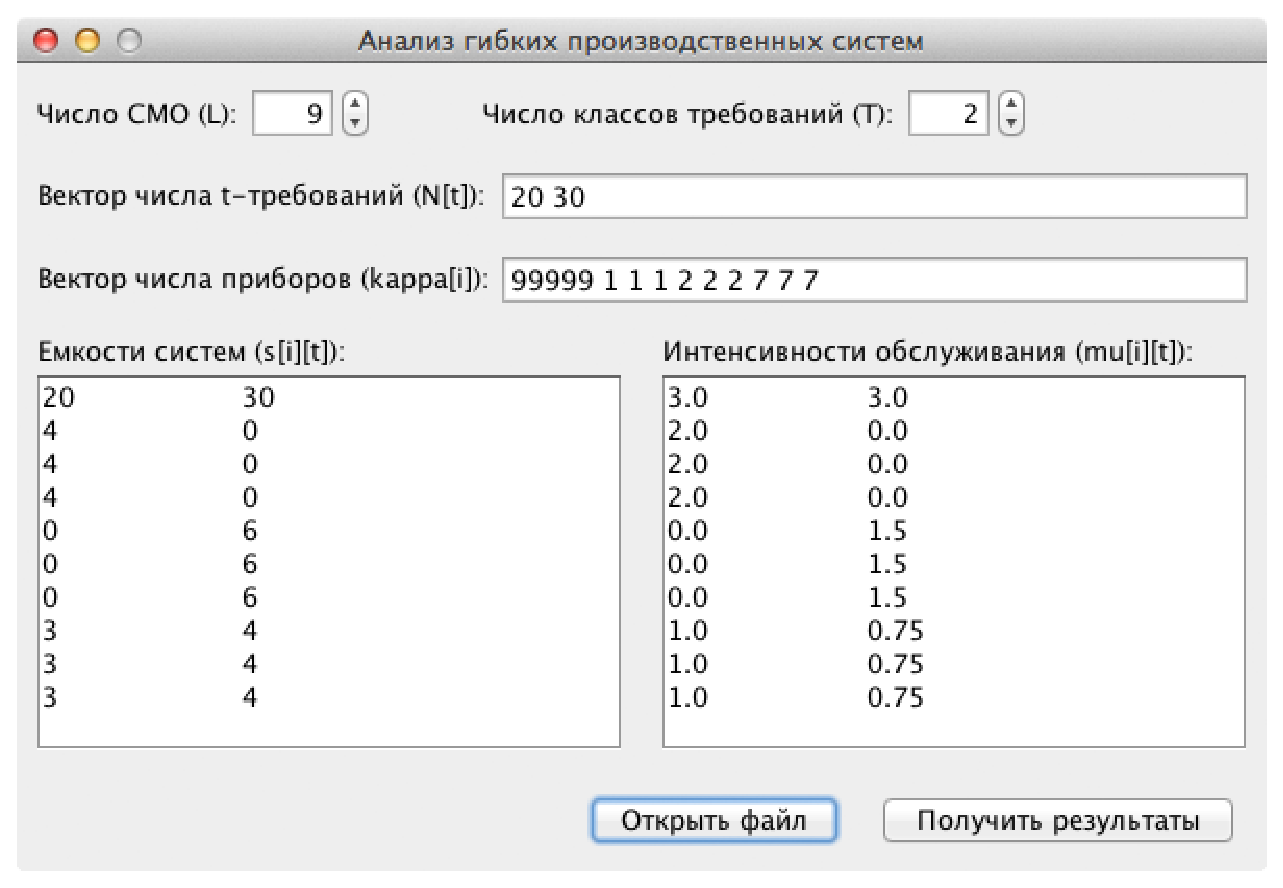
\includegraphics[width=0.9\textwidth]{main}
  \label{fig:main}
\end{figure}
\end{frame}

% ------------------------------------------------------------------- %

\begin{frame} \frametitle{Интерфейс программы}
\begin{figure}[H]
  \centering
  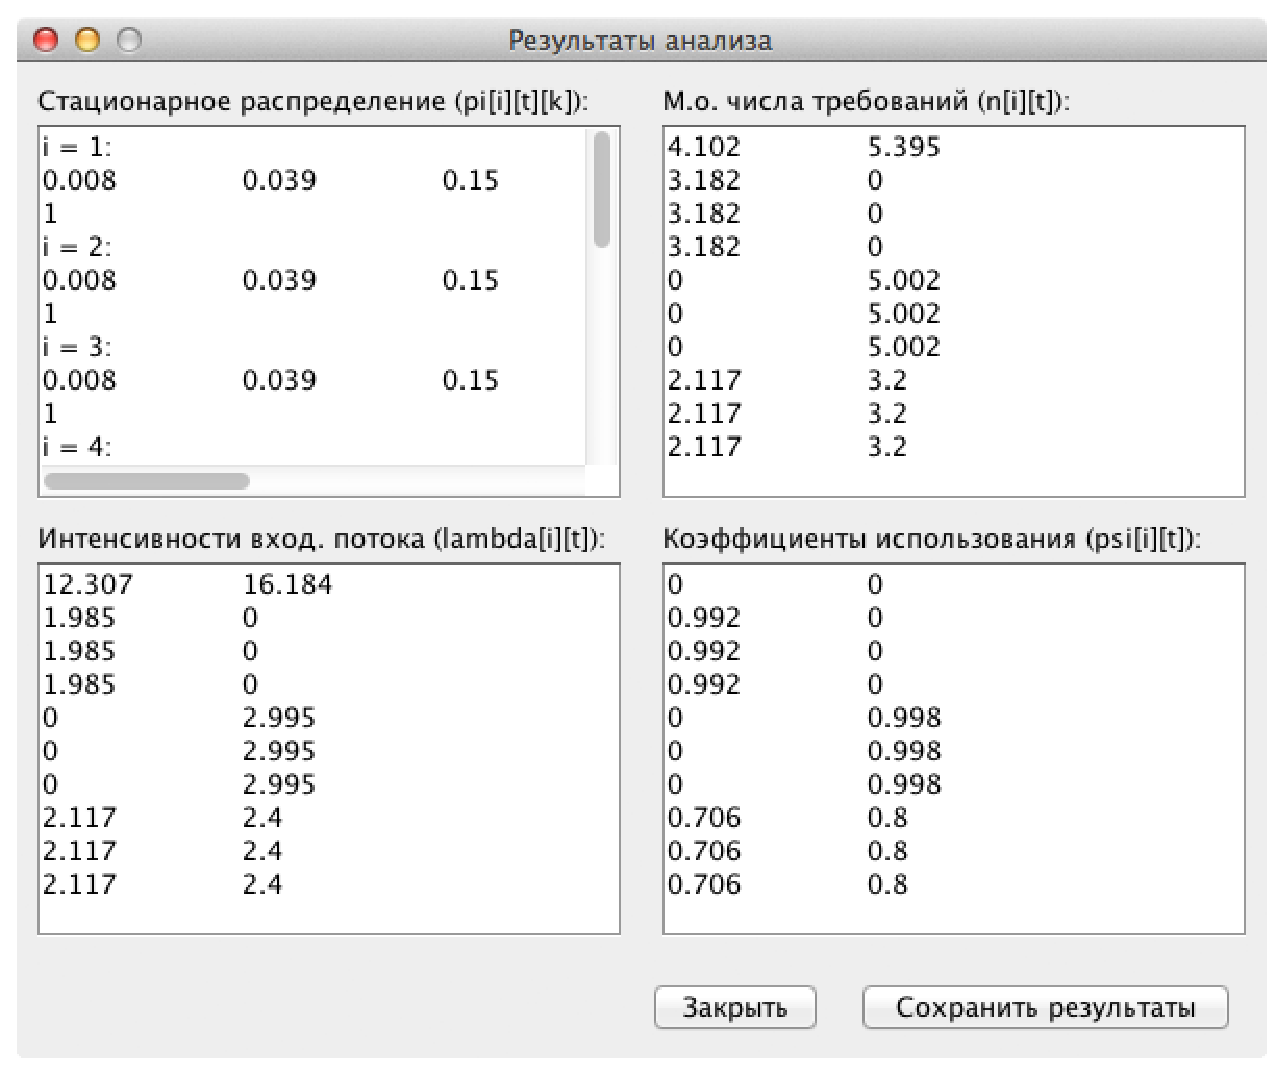
\includegraphics[width=0.8\textwidth]{results}
  \label{fig:main}
\end{figure}
\end{frame}

% ------------------------------------------------------------------- %

\begin{frame} \frametitle{Эксперимент 1}
Рассмотрим производственную систему с $18$ машинами, которые сгруппированы по $9$ рабочим станциям. Число приборов, интенсивность обработки детали одним прибором и емкость локального хранилища на каждой станции соответственно равны: \\
$\kappa_1=\kappa_2=\kappa_3=1$; $\kappa_4=\kappa_5=\kappa_6=2$; $\kappa_7=\kappa_8=\kappa_9=3$; \\
$\mu_1=\mu_2=\mu_3=2$; $\mu_4=\mu_5=\mu_6=1,5$; $\mu_7=\mu_8=\mu_9=1$; \\
$s_1=s_2=s_3=4$; $s_4=s_5=s_6=6$; $s_7=s_8=s_9=7$. \\

Число транспортеров $\kappa_0=9$, каждый из которых имеет интенсивность обработки $\mu_0=3$. В данной системе есть $N=50$ палет, т.е. общее число деталей (одного типа) в любой момент времени равно $50$.
\end{frame}

% ------------------------------------------------------------------- %

\begin{frame} \frametitle{Эксперимент 1}
Математическое ожидание числа деталей ($\overline{n}_i$), пропускная способность ($\lambda_i$) и коэффициенты использования приборов ($\psi_i$) для каждой станции:

{\renewcommand{\arraystretch}{1.5}%
\begin{table}[H]
\begin{tabular}{|c|c|c|c|c|}
\hline
$C_i$ & $C_0$ & $C_{1, 2, 3}$ & $C_{4, 5, 6}$ & $C_{7, 8, 9}$ \cr
\hline
$\overline{n}_i$  &  11,070  &  3,003  &  4,492  &  5,482 \cr
\hline
$\lambda_i$  &  23,595  &  1,954  &  2,950  &  2,961 \cr
\hline
$\psi_i$  &  0,874  &  0,977  &  0,983  &  0,987 \cr
\hline
\end{tabular}
\end{table}}
\end{frame}

% ------------------------------------------------------------------- %

\begin{frame} \frametitle{Эксперимент 2. Зависимость стационарных характеристик ГПС от числа приборов}
\begin{figure}[H]
  \centering
  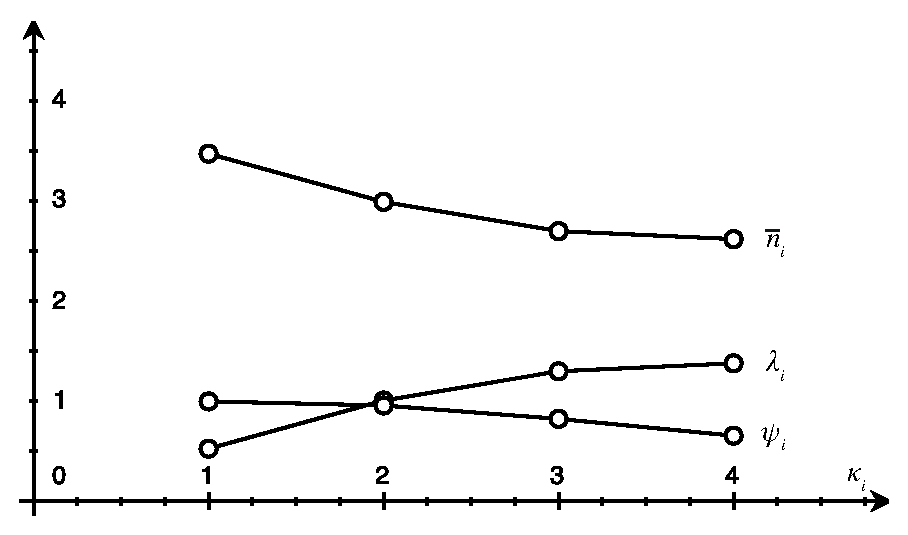
\includegraphics[width=0.9\textwidth]{graph1}
  \label{fig:main}
\end{figure}
\end{frame}

% ------------------------------------------------------------------- %

\begin{frame} \frametitle{Эксперимент 2. Зависимость стационарных характеристик ГПС от емкостей рабочих станций}
\begin{figure}[H]
  \centering
  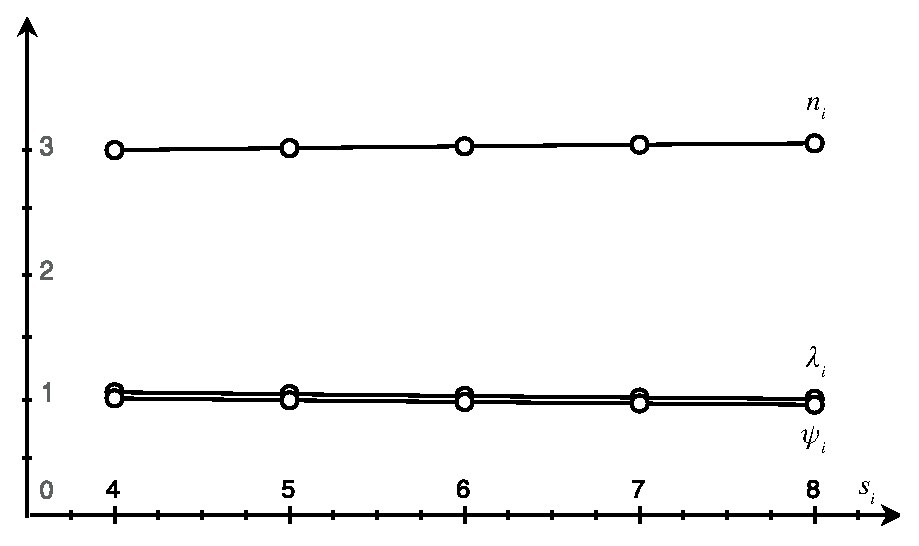
\includegraphics[width=0.9\textwidth]{graph2}
  \label{fig:main}
\end{figure}
\end{frame}

% ------------------------------------------------------------------- %

\begin{frame} \frametitle{Эксперимент 2. Зависимость стационарных характеристик ГПС от интенсивностей обработки деталей}
\begin{figure}[H]
  \centering
  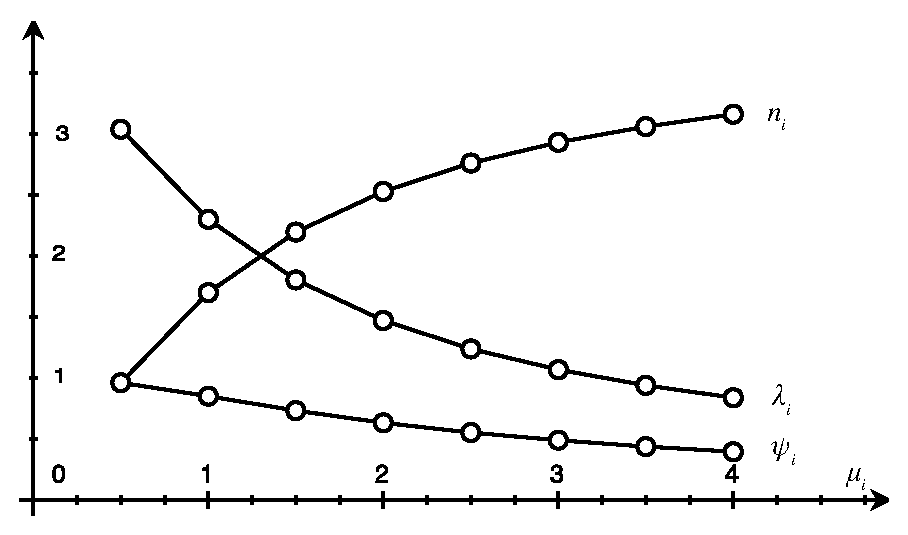
\includegraphics[width=0.9\textwidth]{graph3}
  \label{fig:main}
\end{figure}
\end{frame}
